\documentclass[a4paper]{article}
\usepackage[english]{babel}
%\usepackage{simplemargins}

%\usepackage[square]{natbib}
\usepackage{amsmath}
\usepackage{amsfonts}
\usepackage{amssymb}
\usepackage{bbold}
\usepackage{graphicx}
\usepackage{blindtext}
\usepackage{hyperref}
\usepackage{amsthm}
\newtheorem{theorem}{Theorem}
\newtheorem{lemma}{Lemma}
\usepackage{algorithm}
%\usepackage{algorithmic}
\usepackage{algpseudocode}
%\usepackage{algorithm2e}
\usepackage{booktabs}

\setcounter{MaxMatrixCols}{20}

\begin{document}
\pagenumbering{arabic}

\Large
 \begin{center}
Finite Difference Method for Elliptic Equations\\


\hspace{10pt}

% Author names and affiliations
\large
%Lic. Julio A. Medina$^1$ \\
Julio A. Medina\\
\hspace{10pt}
\small  
Universidad de San Carlos\\
School of Physical and Mathematical Sciences\\
Master's Program in Physics\\
\href{mailto:julioantonio.medina@gmail.com}{julioantonio.medina@gmail.com}\\

\end{center}

\hspace{10pt}

\normalsize
\section{Elliptic partial differential equations}
The elliptic partial differential equation considered in this work is Poisson's equation
\begin{equation}\label{eq::Poisson}
\nabla^2 u(x,y)\equiv \frac{\partial^2 u}{\partial x^2}(x,y) + \frac{\partial^2 u}{\partial y^2}(x,y)=f(x,y)
\end{equation}
in $R=\{ (x,y)\,\,|\,\, a<x<b ,\, c<y<d \}$, with $u(x,y)=g(x,y) \in S$, where $S$ denotes the boundary of $R$. If $f$ and $g$ are continuous on their domains, then the equation has a unique solution.

\subsection{Choosing a mesh}
The method used here is a two-dimensional adaptation of the finite difference method for problems with linear boundaries, as discussed in \cite{Burden}. The first step is to choose integers $n$ and $m$ in order to define the step sizes $h=(b-a)/n$ and $k=(d-c)/m$. In this way, the interval $[a,b]$ is partitioned into $n$ equal parts of width $h$, and the interval $[c,d]$ is partitioned into $m$ equal parts of width $k$, forming a mesh or grid as shown in the figure.

\begin{figure}[h]
\begin{center}\label{fig::mesh}
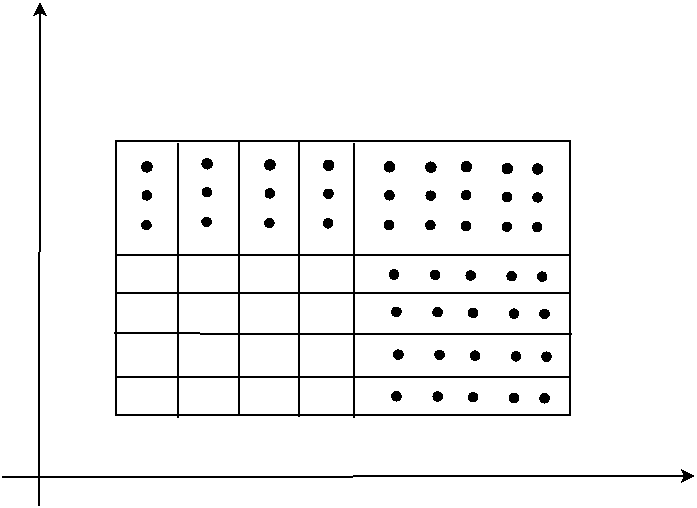
\includegraphics[scale=0.25]{./lattice.png} 
\end{center} 
\caption{$n\times m$ grid}
\end{figure}
This mesh is formally constructed by drawing vertical and horizontal lines over the rectangle $R$ at the points with coordinates $(x_i, y_j)$, where
\begin{equation}
x_i=a+ih,\,\,\,\text{for each }i=0,1,2,\hdots,n\, \text{ and }\, y_j=c+jk,\,\,\,\text{for each }j=0,1,2,\hdots,m.
\end{equation}
The lines corresponding to $x=x_i$ and $y=y_j$ form the grid, and their intersections are the mesh points. For each interior mesh point $(x_i,y_j)$, with $i=1,2,\hdots,n-1$ and $j=1,2,\hdots,m-1$, a Taylor series in the variable $x$ around the point $x_i$ can be used to generate the centered-difference formula
\begin{equation}
\frac{\partial^2 u}{\partial x^2}(x_i,y_j)=\frac{u(x_{i+1},y_j)-2u(x_i,y_j)+u(x_{i-1},y_j)}{h^2}-\frac{h^2}{12}\frac{\partial^4 u}{\partial x^4}(\xi_i,y_j)
\end{equation}
where $\xi_i \in (x_{i-1},x_{i+1})$. Similarly, using the Taylor series in the variable $y$ around the point $y_j$, one obtains the centered difference
\begin{equation}
\frac{\partial^2 u}{\partial y^2}(x_i,y_j)=\frac{u(x_{i},y_{j+1})-2u(x_i,y_j)+u(x_{i},y_{j-1})}{k^2}-\frac{k^2}{12}\frac{\partial^4 u}{\partial y^4}(x_i,\eta_j)
\end{equation}
where $\eta_j \in (y_{j-1},y_{j+1})$. Substituting these formulas into equation \ref{eq::Poisson} allows Poisson's equation to be written at the points $(x_i,y_j)$ as
\begin{equation}
\begin{aligned}
&\frac{u(x_{i+1},y_j)-2u(x_i,y_j)+u(x_{i-1},y_j)}{h^2}+\frac{u(x_{i},y_{j+1})-2u(x_i,y_j)+u(x_{i},y_{j-1})}{k^2}\\
&=f(x_i,y_j)+\frac{h^2}{12}\frac{\partial^4 u}{\partial x^4}(\xi_i,y_j)+\frac{k^2}{12}\frac{\partial^4 u}{\partial y^4}(x_i,\eta_j)
\end{aligned}
\end{equation}
for each $i=1,2,\hdots,n-1$ and $j=1,2,\hdots,m-1$. The boundary conditions are
\begin{equation*}
u(x_0,y_j)=g(x_0,y_j)\,\, \text{ and } \,\, u(x_n,y_j)=g(x_n,y_j),\,\,\, \text{for each }j=0,1,\hdots,m;
\end{equation*}
\begin{equation*}
u(x_i,y_0)=g(x_i,y_0)\,\, \text{ and } \,\, u(x_i,y_m)=g(x_i,y_m),\,\,\, \text{for each }i=1,2,\hdots,n-1.
\end{equation*}

\subsection{Finite Difference Method}
In difference-equation form, the finite difference method is
\begin{equation}\label{eq::finite_difference}
2\Bigg[\Bigg(\frac{h}{k}\Bigg)^2 +1  \Bigg]w_{ij}-(w_{i+1,j}+w_{i-1,j})-\Bigg(\frac{h}{k}\Bigg)^2(w_{i,j+1}+w_{i,j-1})=-h^2 f(x_i,y_j)
\end{equation}
for each $i=1,2,\hdots,n-1$ and $j=1,2,\hdots,m-1$, where
\begin{equation}\label{eq:boundary_conditions}
\begin{aligned}
&w_{0j}=g(x_0,y_j)\,\,\text{and }\, w_{nj}=g(x_n,y_j),\,\,\, \text{for each } j=0,1,\hdots,m;\\
&w_{i0}=g(x_i,y_0)\,\,\text{and }\, w_{im}=g(x_i,y_m),\,\,\, \text{for each } i=1,2,\hdots,n-1.
\end{aligned}
\end{equation}
Here, $w_{ij}$ approximates $u(x_i,y_j)$. This method has a truncation error of order $O(h^2+k^2)$. Equation \ref{eq::finite_difference} involves approximations to $u(x,y)$ at the points
\begin{equation*}
(x_{i-1},y_{j}),\,\,\,(x_{i+1},y_{j}),\,\,\,(x_{i},y_{j}),\,\,\,(x_{i},y_{j-1}),\,\text{and}\,\,(x_{i},y_{j+1}).\,\,\,
\end{equation*}
Using the information provided by the boundary conditions \ref{eq:boundary_conditions} whenever the system defined by \ref{eq::finite_difference} allows it, that is, at the points adjacent to the boundary defined by the previously constructed grid (\ref{fig::mesh}), one obtains a system of equations with a coefficient matrix of dimension $(n-1)(m-1)\times(n-1)(m-1)$. The unknowns are the approximations $w_{ij}$ to $u(x_i,y_j)$ at the interior mesh points (\ref{fig::mesh}).\\

The linear system for the unknowns $w_{ij}$ can be represented more efficiently for matrix operations by relabeling the interior mesh points. A recommended relabeling scheme can be found in \cite{Varga} and is defined as follows:
\begin{equation}
P_l=(x_i,y_j), \,\,\, \text{and}\,\,\, w_l=w_{ij},
\end{equation}
where
\begin{equation}\label{eq::relabeling_function}
l(i,j)=i+(m-1-j)(n-1)
\end{equation} 
for each $i=1,2,\hdots,n-1$ and $j=1,2,\hdots,m-1$. With this scheme, the interior mesh points are labeled from left to right and from top to bottom. This ensures that the resulting linear system for finding $w_{ij}$ has a banded matrix with maximum bandwidth $2n-1$, specifically a block-tridiagonal matrix. This technique was used to implement the algorithm in Python; see algorithms \ref{alg::funcL} and \ref{alg::finite_difference}.



\section{Finite Difference Method Algorithm for Poisson's Equation}
To obtain an algorithm that generates and solves the finite difference method for the elliptic partial differential equations described in the previous section, the relabeling scheme introduced above is used. This ensures that a block-tridiagonal system is obtained. For these block-tridiagonal systems, it is convenient to apply a generalization of the Crout factorization algorithm \cite{Varga} for block-tridiagonal matrices.\\
Another iterative algorithm that can be used is the SOR relaxation method. With this in mind, a strategy for constructing a finite difference algorithm can be outlined as follows:
\begin{itemize}
\item Construct the system associated with the approximations $w_{ij}$ to $u(x_i,y_j)$ using the relabeling scheme presented above.
\item Apply a method for solving linear systems: the generalized Crout factorization or the iterative SOR method.
\item Solve for $w_{ij}$.
\end{itemize}

\subsection{Finite difference algorithm: linear system}
\subsubsection{Relabeling function $l$}
The function $l$ is implemented to relabel the linear system of equations.
\begin{algorithm}[H]
\caption{Function $L$ for relabeling the variables of the linear system}\label{alg::funcL}
\begin{algorithmic}[H]
\Function L {$i, j, n, m$}
\State \Return $(i+1) + (m-1-(j+1)) \times (n-1) - 1$
\EndFunction
\end{algorithmic}
\end{algorithm}

\subsubsection{Associated linear system}
With this function, the system associated with the finite difference method is created.
\begin{algorithm}[H]
\caption{Finite Difference Linear System}\label{alg::finite_difference}
\begin{algorithmic}[H]
\Function{finite\_difference\_linear\_system}{$a,b,c,d,n,m,f,g$}
\State $h \gets (b-a)/n$
\State $k \gets (d-c)/m$
\State $x \gets \text{numpy.linspace}(a, b, n+1)$
\State $y \gets \text{numpy.linspace}(c, d, m+1)$
\State $W_{ij} \gets$ zeros $(((n-1)\times(m-1)),((n-1)\times(m-1)))$
\State $w \gets$ zeros $((n-1)\times(m-1))$
\For{$i \gets 0$ to $n-2$}
\For{$j \gets 0$ to $m-2$}
\State $W_{ij}[L(i,j,n,m), L(i,j,n,m)] \gets 2((h/k)^2 + 1)$
\If{$i \neq 0$ and $i \neq n-2$}
\State $W_{ij}[L(i,j,n,m), L(i+1,j,n,m)] \gets -1$
\State $W_{ij}[L(i,j,n,m), L(i-1,j,n,m)] \gets -1$
\Else
\If{$i = 0$}
\State $W_{ij}[L(i,j,n,m), L(i+1,j,n,m)] \gets -1$
\State $w[l(i,j,n,m)] \gets g(x[i], y[j+1], a, b, c, d)$
\EndIf
\If{$i = n-2$}
\State $W_{ij}[L(i,j,n,m), L(i-1,j,n,m)] \gets -1$
\State $w[L(i,j,n,m)] \gets g(x[i+2], y[j+1], a, b, c, d)$
\EndIf
\EndIf
\If{$j \neq 0$ and $j \neq m-2$}
\State $W_{ij}[L(i,j,n,m), L(i,j+1,n,m)] \gets-(h/k)^2$
\State $W_{ij}[L(i,j,n,m), L(i,j-1,n,m)] \gets-(h/k)^2$
\Else
\If{$j = 0$}
\State $W_{ij}[L(i,j,n,m), L(i,j+1,n,m)] \gets -(h/k)^2$
\State $aux\gets (h/k)^2*g(x[i+1],y[j],a,b,c,d)$
\State $w[L(i,j,n,m)] \gets w[L(i,j,n,m)]+ aux$
\EndIf
\If{$j = m-2$}
\State $W_{ij}[L(i,j,n,m), L(i,j-1,n,m)] \gets -(h/k)^2$
\State $aux\gets (h/k)^2*g(x[i+1],y[j+2],a,b,c,d)$
\State $w[L(i,j,n,m)] \gets w[L(i,j,n,m)]+ aux$
\EndIf
\EndIf
\State $w[L(i,j,n,m)] \gets-h^2f(x[i+1],y[j+1])+w[L(i,j,n,m)]$
\EndFor
\EndFor
\State \textbf{return} $W_{ij}, w$
\EndFunction
\end{algorithmic}
\end{algorithm}

\subsection{Generalized Crout factorization algorithm for block-tridiagonal matrices}
This is the implementation of the generalized Crout factorization algorithm for block-tridiagonal matrices. The standard Crout factorization algorithm is valid for tridiagonal matrices, but not directly for block-tridiagonal matrices.
\begin{algorithm}[H]
\caption{Crout Generalization Algorithm for Tridiagonal Block Matrices}\label{alg::Crout}
\begin{algorithmic}[H]
\Require $A \in \mathbb{R}^{N \times N}$, $K \in \mathbb{R}^{N}$, $n \in \mathbb{N}$
\Ensure $sol \in \mathbb{R}^{N}$
\Function{Crout\_generalization}{$A, K, n$}
\State $N \gets \lfloor \frac{\operatorname{shape}(A)[1]}{n} \rfloor$
\State $W \gets []$
\State $B_1 \gets A_{1:n,1:n}$
\State $C_1 \gets A_{1:n,n:n+n}$
\State $W.append(\operatorname{inv}(B_1) \cdot C_1)$
\For{$i \gets 2$ to $N-1$}
\State $B_i \gets A_{(i-1)n:in,(i-1)n:in}$
\State $A_i \gets A_{(i-1)n:in,(i-2)n:(i-1)n}$
\State $C_i \gets A_{(i-1)n:in,in+1:n+(i-1)n}$
\State $W.append(\operatorname{inv}(B_i - A_i \cdot W_{i-2}) \cdot C_i)$
\EndFor
\State $B_N \gets A_{1:n,1:n}$
\State $K_1 \gets K_{1:n}$
\State $G_1 \gets \operatorname{inv}(B_1) \cdot K_1$
\State $G \gets []$
\State $G.append(G_1)$
\For{$i \gets 2$ to $N$}
\State $K_i \gets K_{(i-1)n:in}$
\State $B_i \gets A_{(i-1)n:in,(i-1)n:in}$
\State $A_i \gets A_{(i-1)n:in,(i-2)n:(i-1)n}$
\State $G.append(\operatorname{inv}(B_i - A_i \cdot W_{i-2}) \cdot (K_i - A_i \cdot G_{i-2}))$
\EndFor
\State $Z \gets G[:]$
\For{$i \gets N-2$ to $0$ step $-1$}
\State $Z_i \gets G_i - W_i \cdot Z_{i+1}$
\EndFor
\State $sol \gets \operatorname{concatenate}(Z)$
\State \textbf{return} $sol$
\EndFunction
\end{algorithmic}
\end{algorithm}

\subsection{Iterative SOR method for solving linear systems}
\begin{algorithm}[H]
\caption{Iterative SOR method for solving linear systems}\label{alg::SOR}
\begin{algorithmic}[H]
\Require{$A$ is an $n \times n$ matrix, $b$ is a right-hand-side vector of dimension $n$, $x^{(0)}$ is an initial proposed solution, $\omega$ is the relaxation parameter, $\epsilon$ is the tolerance, and $max_{iter}$ is the maximum number of iterations.}
\Ensure{$x$ is an approximate solution of $Ax = b$.}
\Function{SOR}{$A,b,\omega,\epsilon,\max_{iter},x^{(0)}$}
\State $k \gets 1$
\State $xo \gets x^{(0)}$
\State $tolerance\gets \textbf{True}$
\While{$k < max_{iter}$ and $\text{tolerance}$}
\For{$i = 1$ to $n$}
\State $s \gets \sum_{j=1}^{i-1} a_{ij}x_j + \sum_{j=i+1}^{n} a_{ij}xo_j$
\State $x_i \gets (1-\omega) xo_i + \frac{\omega}{a_{ii}} (b_i - s)$
\EndFor
\If{$||x - xo|| < \epsilon$}
\State $tolerance\gets \textbf{False}$
\EndIf
\State $k \gets k+1$
\State $xo=x$
\EndWhile
\If{$k = max_{iter}$}
\State \textbf{print} ``The maximum number of iterations has been reached''
\EndIf
\State \textbf{return} $x$
\EndFunction
\end{algorithmic}
\end{algorithm}

\subsection{Finite differences using generalized Crout factorization}
\begin{algorithm}[H]
\caption{Finite difference algorithm using generalized Crout factorization}\label{alg::finite_diff_Crout}
Given a problem with boundary conditions of the form \ref{eq::Poisson}, define
\begin{equation*}
a,b,c,d,n,m,f(x,y),g(x,y)
\end{equation*}
using the functions defined in algorithms \ref{alg::finite_difference} and \ref{alg::Crout}.
\begin{algorithmic}
%\State use the function defined in the algorithm 
\State $A, b\gets$ finite\_difference\_linear\_system$(a,b,c,d,n,m,f,g)$
%\State use the function defined in the algorithm 
\State $solution\gets $ Crout\_generalization(A,b,n-1)
\end{algorithmic}
\end{algorithm}
This algorithm was implemented in Python using the NumPy library. The repository can be found at \url{https://github.com/Julio-Medina/Finite_Difference_Method/tree/main/code}.

\subsection{Finite differences using the SOR relaxation method}
\begin{algorithm}[H]
\caption{Finite difference algorithm using the SOR relaxation method}\label{alg::finite_diff_SOR}
Given a problem with boundary conditions of the form \ref{eq::Poisson}, define
\begin{equation*}
a,b,c,d,n,m,f(x,y),g(x,y),\omega,\epsilon,x^{(0)}
\end{equation*}
using the functions defined in algorithms \ref{alg::finite_difference} and \ref{alg::SOR}.
\begin{algorithmic}
%\State use the function defined in the algorithm 
\State $A, b\gets$ finite\_difference\_linear\_system$(a,b,c,d,n,m,f,g)$
%\State use the function defined in the algorithm 
\State $solution\gets $ SOR($A,b,\omega,\epsilon,\max_{iter},x^{(0)}$)
\end{algorithmic}
\end{algorithm}

\subsection{Examples}
There is no better way to illustrate how the algorithm works than by solving some boundary-value problems.

\subsubsection{Example 1}
Solve the following problem:
\begin{equation}
\frac{\partial^2 u}{\partial x^2}(x,y)+\frac{\partial^2 u}{\partial y^2}(x,y)=0
\end{equation}
for each $(x,y)$ in the set $R=\{ (x,y)|\, 0<x<0.5,\, 0<y<0.5 \}$. The boundary conditions are
\begin{equation*}
u(0,y)=0,\,u(x,0)=0,\, u(x,0.5)=200x,\, u(0.5,y)=200y.\,
\end{equation*}
If $n=m=4$, the finite difference equation \ref{eq::finite_difference} gives
\begin{equation}
4w_{i,j}-w_{i+1,j}-w_{i-1,j}-w_{i,j-1}-w_{i,j+1}=0
\end{equation}
for each $i=1,2,3$ and $j=1,2,3$.\\
For example, when $i=1,j=1$, one obtains
\begin{equation}\label{eq::finite_diff1}
4w_{1,1}-w_{2,1}-w_{0,1}-w_{1,0}-w_{1,2}=0.
\end{equation}
Since $w_{1,0}=w_{0,1}=0$, using the relabeling function \ref{eq::relabeling_function} gives
\begin{equation*}
l(1,1)=7,\,l(2,1)=8,\,l(1,2)=4.
\end{equation*}
Substituting into \ref{eq::finite_diff1} and using the boundary conditions gives the equation
\begin{equation*}
4w_{7}-w_{8}-w_{4}=0.
\end{equation*}
This process is repeated for the remaining indices, producing $9$ linear equations for the variables $w_1,w_2,w_3,w_4,w_5,w_6,w_7,w_8,w_9$. The coefficient matrix of the linear system obtained by iterating through all indices is
\begin{equation}\label{eq::block_tridiagonal_matrix_1}
A =
\begin{bmatrix}
4.0 & -1.0 & 0.0 & -1.0 & 0.0 & 0.0 & 0.0 & 0.0 & 0.0 \\
-1.0 & 4.0 & -1.0 & 0.0 & -1.0 & 0.0 & 0.0 & 0.0 & 0.0 \\
0.0 & -1.0 & 4.0 & 0.0 & 0.0 & -1.0 & 0.0 & 0.0 & 0.0 \\
-1.0 & 0.0 & 0.0 & 4.0 & -1.0 & 0.0 & -1.0 & 0.0 & 0.0 \\
0.0 & -1.0 & 0.0 & -1.0 & 4.0 & -1.0 & 0.0 & -1.0 & 0.0 \\
0.0 & 0.0 & -1.0 & 0.0 & -1.0 & 4.0 & 0.0 & 0.0 & -1.0 \\
0.0 & 0.0 & 0.0 & -1.0 & 0.0 & 0.0 & 4.0 & -1.0 & 0.0 \\
0.0 & 0.0 & 0.0 & 0.0 & -1.0 & 0.0 & -1.0 & 4.0 & -1.0 \\
0.0 & 0.0 & 0.0 & 0.0 & 0.0 & -1.0 & 0.0 & -1.0 & 4.0 \\
\end{bmatrix}
\end{equation}
and the constant vector is
\begin{equation*}
b =
\begin{bmatrix}
25.0 \\
50.0 \\
150.0 \\
0.0 \\
0.0 \\
50.0 \\
0.0 \\
0.0 \\
25.0 \\
\end{bmatrix}.
\end{equation*}
It is important to note that the resulting matrix \ref{eq::block_tridiagonal_matrix_1} is a block-tridiagonal matrix, with each block having dimension $3\times 3$. Thus, the system
\begin{equation}
Aw=b
\end{equation}
can be solved, giving
\begin{equation}
\begin{bmatrix}
w_1 \\
w_2 \\
w_3 \\
w_4 \\
w_5 \\
w_6 \\
w_7 \\
w_8 \\
w_9 \\
\end{bmatrix}=
\begin{bmatrix}
18.75 \\
37.5 \\
56.25 \\
12.5 \\
25 \\
37.5 \\
6.25 \\
12.5 \\
18.75 \\
\end{bmatrix}.
\end{equation}

\subsubsection{Example 2}
Solve the following problem:
\begin{equation}
\frac{\partial^2 u}{\partial x^2}(x,y)+\frac{\partial^2 u}{\partial y^2}(x,y)=4
\end{equation}
for each $(x,y)$ in the set $R=\{ (x,y)|\, 0<x<1,\, 0<y<2 \}$. The boundary conditions are
\begin{equation*}
u(1,y)=\ln(y^2+1),\,u(x,0)=2\ln x,\, u(x,1)=\ln(x^2+1),\, u(2,y)=\ln(y^2+4).
\end{equation*}
If $h=k=\frac{1}{3}$, then $n=3,\,\,m=3$, and the finite difference equation \ref{eq::finite_difference} gives
\begin{equation}
4w_{i,j}-w_{i+1,j}-w_{i-1,j}-w_{i,j-1}-w_{i,j+1}=4.
\end{equation}
The associated coefficient matrix $A$ is
\begin{equation}\label{eq::block_tridiagonal_matrix_2}
\begin{bmatrix}
 4.0 & -1.0 &  -1.0 &  0.0\\
 -1.0 & 4.0 &  0.0 &  -1.0\\
 -1.0 & 0.0 &  4.0 &  -1.0\\
 0.0 & -1.0 &  -1.0 &  4.0\\    
\end{bmatrix}
\end{equation}
and the constant vector is
\begin{equation*}
b =
\begin{bmatrix}
 1.165 \\
 2.774 \\
 -0.444 \\
 1.165 \\
\end{bmatrix}.
\end{equation*}
It is important to note that the resulting matrix \ref{eq::block_tridiagonal_matrix_2} is a block-tridiagonal matrix, with each block having dimension $2\times 2$. Thus, the system
\begin{equation}
Aw=b
\end{equation}
can be solved, giving
\begin{equation}
\begin{bmatrix}
w_1 \\
w_2 \\
w_3 \\
w_4 \\
\end{bmatrix}=
\begin{bmatrix}
  0.5825 \\
 0.9849 \\
 0.1801 \\
 0.5825 \\
\end{bmatrix}.
\end{equation}

\subsubsection{Example 3}
Solve the following problem:
\begin{equation}
\frac{\partial^2 u}{\partial x^2}(x,y)+\frac{\partial^2 u}{\partial y^2}(x,y)=x e^{y}
\end{equation}
for each $(x,y)$ in the set $R=\{ (x,y)|\, 0<x<2,\, 0<y<1 \}$. The boundary conditions are
\begin{equation*}
u(0,y)=0,\,u(x,0)=x,\, u(x,1)=ex,\, u(2,y)=2e^y.
\end{equation*}
With $n=6,\,\,m=5$, compare the approximations with the analytical solution $u(x,y)=x e^y$.\\
Using the functions created in Python gives the following table. This table can be found in the GitHub repository mentioned above under the name \texttt{error\_table.csv}.\\
\begin{tabular}{lrrrrrrr}
\toprule
{} &  $i$ &  $j$ &       $x_i$ &  $y_j$ &      $w_{ij}$ &  $u(x_i,y_j)$ &  $|u(x_i,y_j)-w_{ij}|$ \\
\midrule
0  &  1 &  1 &  0.333333 &  0.2 &  0.407265 &    0.407134 &           0.000130 \\
1  &  1 &  2 &  0.333333 &  0.4 &  0.497483 &    0.497275 &           0.000208 \\
2  &  1 &  3 &  0.333333 &  0.6 &  0.607596 &    0.607373 &           0.000223 \\
3  &  1 &  4 &  0.333333 &  0.8 &  0.742007 &    0.741847 &           0.000160 \\
4  &  2 &  1 &  0.666667 &  0.2 &  0.814524 &    0.814269 &           0.000255 \\
5  &  2 &  2 &  0.666667 &  0.4 &  0.994958 &    0.994550 &           0.000408 \\
6  &  2 &  3 &  0.666667 &  0.6 &  1.215183 &    1.214746 &           0.000437 \\
7  &  2 &  4 &  0.666667 &  0.8 &  1.484009 &    1.483694 &           0.000315 \\
8  &  3 &  1 &  1.000000 &  0.2 &  1.221766 &    1.221403 &           0.000363 \\
9  &  3 &  2 &  1.000000 &  0.4 &  1.492405 &    1.491825 &           0.000580 \\
10 &  3 &  3 &  1.000000 &  0.6 &  1.822743 &    1.822119 &           0.000624 \\
11 &  3 &  4 &  1.000000 &  0.8 &  2.225993 &    2.225541 &           0.000452 \\
12 &  4 &  1 &  1.333333 &  0.2 &  1.628964 &    1.628537 &           0.000427 \\
13 &  4 &  2 &  1.333333 &  0.4 &  1.989778 &    1.989100 &           0.000679 \\
14 &  4 &  3 &  1.333333 &  0.6 &  2.430227 &    2.429492 &           0.000735 \\
15 &  4 &  4 &  1.333333 &  0.8 &  2.967928 &    2.967388 &           0.000540 \\
16 &  5 &  1 &  1.666667 &  0.2 &  2.036042 &    2.035671 &           0.000371 \\
17 &  5 &  2 &  1.666667 &  0.4 &  2.486958 &    2.486374 &           0.000584 \\
18 &  5 &  3 &  1.666667 &  0.6 &  3.037506 &    3.036865 &           0.000641 \\
19 &  5 &  4 &  1.666667 &  0.8 &  3.709724 &    3.709235 &           0.000489 \\
\bottomrule
\end{tabular}




\begin{thebibliography}{99}
%% The bibliography is ordered alphabetically by the surname of the author
%% or main author. Each entry has its own format depending on whether it is
%% a book, article, thesis, web content, etc.


\bibitem{Burden} Richard L. Burden, J. Douglas Faires \textit{Numerical Analysis}, (Ninth Edition). Brooks/Cole, Cengage Learning. 978-0-538-73351-9

\bibitem{Varga} Richard S. Varga. \textit{Matrix Iterative Analysis}. Second Edition. Springer. DOI 10.1007/978-3-642-05156-2

%\bibitem{Feynman} 
%\bibitem{Hopfield} J.J. Hopfield. \textit{Neural Networks and physical systems with emergent collective computational abilities}. \url{https://doi.org/10.1073/pnas.79.8.2554}


%\bibitem{McCulloch} Warren S. McChulloch, Walter H. Pitts. \textit{A LOGICAL CALCULUS OF THE IDEAS IMMANENT IN NERVOUS ACTIVITY}. \url{http://www.cse.chalmers.se/~coquand/AUTOMATA/mcp.pdf}



\end{thebibliography}
\end{document}
